\documentclass{llncs}

\usepackage{llncsdoc}

%% PDFLaTeX
% \usepackage[T1]{fontenc}
\usepackage[utf8]{inputenc}
\usepackage{textcomp}      % for ° symbol

\usepackage{multirow}
\usepackage{caption}
\usepackage{url}
\usepackage{tabularx}
\usepackage{tikz}
\usetikzlibrary{automata,positioning}

%% XeLaTeX
% \usepackage{fontspec}
% \usepackage{xunicode}
% \usepackage{xltxtra}

\usepackage{expex}

%
\begin{document}
%
\title{HFST---a System for Creating NLP Tools}
%
\author{Krister Lind\'{e}n \and Erik Axelson \and Senka Drobac \and Sam Hardwick \and\\
Juha Kuokkala \and Jyrki Niemi \and Tommi A Pirinen \and Miikka Silfverberg}
% \author{N.N. \and\\
% N.N.}

\institute{University of Helsinki\\
Department of Modern Languages\\
Unioninkatu 40 A\\
FI-00014 University of Helsinki, Finland\\
% \institute{xx\\
% yy\\
% zz\\
% ww\\
\email{\{krister.linden, erik.axelson, senka.drobac, sam.hardwick,\\
juha.kuokkala, jyrki.niemi, tommi.pirinen, miikka.silfverberg\}@helsinki.fi}}
% \email{\{n.n.,\\
% n.n.\}@xxx.yy}}

\maketitle

% Removed the manual bibstyle in favor of splncs03.bst,
% if it's required fetch it from svn history

\begin{abstract}
%Krister
The paper presents and evaluates various NLP tools that have been created using the open source library HFST--Helsinki Finite-State Technology and outlines the minimal extensions that this has required to a pure finite-state system. In particular, the paper describes an implementation and application of Pmatch presented by Karttunen at SFCM 2011.
\keywords{finite-state technology, language identification, morphological guessers, spell-checking, named-entity recognition, language generation, parsing, HFST, XFST, Pmatch}
\end{abstract}

\section*{Introduction}
% Krister
In natural language processing, finite-state string transducer methods have been found useful for solving a number of practical problems ranging from language identification via morphological processing and generation to part-of-speech tagging and named-entity recognition, as long as the problems lend themselves to a formulation based on matching and transforming local context.

% NOTE: repetitive of the abstract
In this paper, we present and evaluate various tools that have been created using HFST--Helsinki Finite-State Technology\footnote{\url{http://hfst.sf.net}} and outline the minimal extensions that this has required to a pure FST system. In particular, we describe an implementation of Pmatch presented by Karttunen at SFCM 2011~\cite{karttunen/2011} and its application to a large-scale named-entity recognizer for Swedish.

The paper is structured as follows: Section~\ref{hfst:structural-layout} is on applications and their evaluation.
In Section~\ref{hfst:env-examples}, we present examples of user environments supported by HFST.
In Section~\ref{hfst:solutions}, we present some of the solutions and extensions needed to implement the applications.
This is followed by the Sections~\ref{hfst:discussion} and \ref{hfst:conclusion} with an outline of some future work and the discussion, respectively.

\section{Applications and Tests}\label{hfst:structural-layout}
In this section, we describe and evaluate some applications implemented with HFST. When processing text corpora, it is useful to first identify the language of the text before analyzing its words morphologically. Words unknown to the morphological lexicon need a guesser derived from the lexicon. The reverse operation of morphological analysis is morphological generation. Generating inflections of words unknown to the morphological lexicon can be used for eliciting information from native speakers before adding the words to the lexicon. For information extraction, it is important to be able to identify multi-word expressions such as named entities, for which purpose HFST has a pattern matching tool. Finally, we also describe a traditional application area of finite-state morphology, i.e. spell-checking and spelling correction, which is now served by a uniform implementation using weighted finite-state technology. 

\subsection{Language identification}
% Miikka
Language identification is the task of recognizing the language of a
text or text fragment. It is useful in applications that need to
process documents written in various languages where the language
might not be explicitly marked in the document. For example, a translation
application might need to identify the language of a document in order
to apply the correct translation model. Another example is a speller
for Finnish, which might need to identify paragraphs written in
English, in order not to spell-check those paragraphs.

In this section we outline how to use HFST tagger tools and language
identification tools for creating language identifiers. We also
present an experiment on language identification for documents written
in Dutch, English, Estonian, Finnish, German or Swedish. The
experiment shows that HFST language identifiers are highly accurate
(99.5\% of the input sentences were correctly classified).

There are several methods for performing language
identification. Highly accurate language identification can be
accomplished by treating data as a letter sequence and training
a Markov chain from training documents whose language is
known~\cite{cavnar/1994}. One Markov chain is trained for each
language that the system recognizes. Language identification consists
of applying each Markov chain on input and choosing the language whose
model gives the highest likelihood for the text. 

HFST language identifiers adopt a Markov chain framework, which can be
implemented with weighted finite-state technology. Using HFST tagger
tools~\cite{silfverberg/2011}, we train Markov models for all
languages. A program, {\tt hfst-guess-language}, reads the
models and input text and labels each sentence with the language
whose model gave the highest likelihood for the sentence.

We present an experiment on applying HFST language identifiers for
guessing the language of sentences written in six languages. For all
languages except Swedish, we used training data from corpora
containing newspaper text. For Swedish, we used more general text.

For Dutch we used the Alpino treebank~\cite{bouma/2000}, for English
we used the Penn Treebank~\cite{marcus/1993}, for Estonian we used the
Estonian National
Corpus\footnote{\url{http://www.cl.ut.ee/korpused/segakorpus/}}, for
Finnish we used text from the largest Finnish newspaper Helsingin
Sanomat year 1995\footnote{\url{http://www.csc.fi/kielipankki/}}, for
German we used the TIGER Corpus~\cite{brants/2002} and for Swedish we
used Talbanken~\cite{einarsson/1976}.

\begin{table}
\small
\begin{center}
\caption{For each language, we used 2000 sentences for training and
  200 sentences for testing. We give the sizes of the data sets in
  utf-8 characters.}\label{tab:lang-id-data}
\begin{tabular}{l|cc}
Language~~~~ & Train data (utf-8 chars) & Test data (utf-8 chars)\\
\hline
Dutch    & 245,000  & 24,000\\
English  & 265,000  & 26,000\\
Estonian & 238,000  & 23,000\\
Finnish  & 155,000  & 14,000\\
German   & 280,000  & 28,000\\
Swedish  & 164,000  & 16,000\\
\hline
\end{tabular}
\end{center}
\end{table}

For each language, we chose 2200 sentences for training and
testing. Of the sentences, every eleventh sentence was used for
testing and the rest for training. This totals 2000 sentences for
training and 200 sentences for testing for each language. The sizes of
the data sets in utf-8 characters are described in
Table~\ref{tab:lang-id-data}. The average length of a sentence in
characters was shorter for Finnish and Swedish than for the other
languages.

\begin{table}
\small
\begin{center}
\caption{We give accuracy of the language guesser per language and for all languages.}\label{tab:lang-id-acc}
\begin{tabular}{ll}
Language~~ & Accuracy\\
\hline
Dutch    & ~~~99.0\%\\
English  & ~~~99.5\%\\
Estonian & ~~~99.5\%\\
Finnish  & ~~~99.5\%\\
German   & ~~100.0\%\\
Swedish  & ~~~99.5\%\\
\hline
ALL      & ~~~99.5\%\\
\hline
\end{tabular}
\end{center}
\end{table}

We ran the language identifier for test sentences from all six
languages (1200 sentences in total) and computed the accuracy of the
language identification system as $corr / all$, where $corr$ is
the number of sentences whose language was correctly guessed and $all$
is the number of all sentences. In Table~\ref{tab:lang-id-acc}, we
show results for each individual language and all the languages
combined. 

Of all sentences, 99.5\% were correctly classified, which demonstrates
that the language identification system is accurate. This is
encouraging because Finnish and Estonian have similar
orthographies. This applies to German, Swedish and Dutch as well.

Currently identification is limited to identifying the closest
language corresponding to a sentence. There is no option to label a
sentence as belonging to an unknown language. 

% It could be possible to
% apply some threshold likelihood $l(n)$ which would state that a model
% has to give a sentence of $n$ characters at least likelihood $l(n)$,
% in order for the sentence to be labeled as belonging to the language
% of the model. 

% In practice it has been very difficult to establish $l(n)$ in a
% reliable way. It is likely to be dependent on the genre of the
% document, which makes it less useful. Identifying unknown language
% using HFST language identifiers thus remains future work.

\subsection{Morphologies and Guessers}
\label{sec: morph-guessers}
% Juha, Miikka

Language technology applications for agglutinating languages such as
Finnish and Hungarian benefit greatly from high-coverage morphological
analyzers, which supply word forms with their morphological
analyses. This makes applications dependent on the coverage of the
morphological analyzer. Building a high-coverage morphological
analyzer (with recall over 95\%) is a substantial task, and even with a
high-coverage analyzer, domain-specific vocabulary presents a
challenge. Therefore, accurate methods for dealing with
out-of-vocabulary words are needed.

With HFST tools it is possible to use an existing morphological
analyzer to construct a morphological guesser based on word
suffixes. Suffix-based guessing is sufficient for many agglutinating
languages such as Finnish~\cite{linden/2009/nodalida}, where most
inflection and derivation is marked using suffixes. Even if a word is
not recognized by the morphological analyzer, the analyzer is likely
to recognize some words which inflect similarly to the unknown
word. These can be used for guessing the inflection of the unknown
word.

The guessing of an unknown word like ``twiitin'' (the genitive form of
``twiitti'', tweet in Finnish) is based on finding recognized word
forms like ``sviitin'' (genitive form of ``sviitti'', hotel suite in
Finnish) that have long suffixes, such as ``-iitin'', which match the
suffixes of the unrecognized word. The longer the common suffix, the
more likely it is that the unrecognized word has the same inflection as
the known word. The guesser will output morphological analyses for
``twiitin'' in order of likelihood.

Besides the length of the matching suffix, guesses can also be ordered
based on the probability that a suffix matches a given analysis. This
can be estimated using a labeled training corpus. In addition, any
existing weighting scheme in the original morphological analyzer can
be utilized.

If the morphological analyzer marks declension class, the guesser can
also be used for guessing the declension class. If the declension
class is marked, the guesser can be used for the generation of word forms
as well as analysis. This is described in Section~\ref{sec:morph-generation}.

\begin{sloppypar}
Constructing a morphological guesser from
OMorFi\footnote{\url{http://code.google.com/p/omorfi/}}--The open-source
Finnish morphology~\cite{pirinen/2008}, the three top guesses for
``twiitin'' are (the markup is slightly simplified): \small
\begin{verbatim}
  twiit  [POS=NOUN] [GUESS_CATEGORY=5]  [NUM=SG][CASE=GEN]
  twiiti [POS=NOUN] [GUESS_CATEGORY=33] [NUM=SG][CASE=NOM]
  twiit  [POS=VERB] [GUESS_CATEGORY=53] [VOICE=ACT][MOOD=INDV] ...
\end{verbatim}
\normalsize
The first field corresponds to the stem of the word, the second field
to its main part of speech and the third to its declension class. The
fourth field shows the inflectional and derivational information of
the guess. In this case, the first guess is correct. It is modeled
after declension class number 5, which is a class of nouns containing
among others the noun ``sviitti''.
\end{sloppypar}

\subsection{Language Generation for Out-of-Vocabulary Words}
\label{sec:morph-generation}
Natural-language user interfaces, such as dialogue systems, need a
language generation component for generating messages for the
user. The aim is to supply the user with information about the
internal state of some database containing information such as airline
connections or weather phenomena.

Language generation systems for agglutinating languages will benefit
from morphological analyzers, because generating syntactically correct
sentences requires inflecting words according to syntactic
context. Depending on the domain and coverage of the morphological
analyzer, it might also be necessary to inflect words that are not
recognized by the morphological analyzer. 

HFST morphological guessers presented in Section~\ref{sec:
  morph-guessers} can be used for generation as well as morphological
analysis. For example, using the OMorFi morphology for Finnish, the
best morphological guess for the unknown word ``twiitin'' is
\begin{verbatim}
  twiit  [POS=NOUN] [GUESS_CATEGORY=5]  [NUM=SG][CASE=GEN]
\end{verbatim}
Replacing the inflectional information {\tt [NUM=SG][CASE=GEN]}
(singular genitive case) by {\tt [NUM=PL][CASE=PAR]} (plural
partitive case) gives the analysis
\begin{verbatim}
  twiit  [POS=NOUN] [GUESS_CATEGORY=5]  [NUM=PL][CASE=PAR]
\end{verbatim}
which can be fed back to the guesser to generate the surface forms
``twiitteja'' and ``twiittejä''. The latter one is correct, though the
first one would also be possible in theory, since the variation
between ``-ja'' and ``-jä'' is governed by Finnish vowel harmony and
the stem ``twiit'' is neutral with respect to vowel harmony.

% Besides language generation, morphological form generation is useful
% when adding new entries to a morphological analyzer. For a human
% expert it is easy to identify whether the word forms in a generated
% list are the correct ones. For frequent words, it is also possible to search a
% corpus for the generated word forms, which can give a clue of whether
% the generated forms constitute actual words and therefore also give a
% clue about whether the guessed morphological analysis is the correct
% one.

\subsection{Extending a lexicon with the help of a guesser}

The morphological guesser has proven to be a useful tool when adding 
large bulks of new vocabulary to a lexicon. We tested this on the Finnish Open Source
lexicon OMorFi. According to our experience with handling ca. 260.000 proper nouns, the guesser achieved
roughly 90\% accuracy in assigning the correct inflection class to new
lexicon entries on the first guess, so the manual work needed was reduced to only
checking the guesser's results and correcting ca. 10\% of the suggested
entries. 

The names to be added to the lexicon were given in their base form, so we
could benefit from accepting only suggestions by the guesser in the nominative case 
\texttt{[CASE=NOM]}. The data was presented to native speakers with key word forms 
generated for each entry, which could be used to distinguish between different inflection classes,
so that it was not necessary to understand the linguistic encoding scheme:
\small
\begin{verbatim}
Aura     9 Aura : Auraa : Aurat : Aurain, Aurojen : Auroja : Auroihin
Oura    10 Oura : Ouraa : Ourat : Ourain, Ourien : Ouria : Ouriin
Pura    10 Pura : Puraa : Purat : Purain, Purien : Puria : Puriin
Saura     9  Saura : Sauraa : Saurat : Saurain, Saurojen : Sauroja : Sauroihin
Peura     9  Peura : Peuraa :  Peurat : Peurain, Peurojen : Peuroja : Peuroihin
Tiura   10 Tiura : Tiuraa : Tiurat : Tiurain, Tiurien : Tiuria : Tiuriin
Heikura 13 Heikura : Heikuraa : Heikurat : Heikurojen, Heikuroiden, 
           Heikuroitten : Heikuroja, Heikuroita : Heikuroihin
\end{verbatim}
\normalsize

%New lexical entries were added to the system in
%several batches and the guesser was rebuilt after each batch. The
%accuracy of the guesser was constantly improving during the process.

We did a preliminary test to assess the accuracy of the guesser when only
some basic proper nouns were included in OMorFi's lexicon. A sample of
100 words from each proper noun list to be added (place names,
companies, organizations, given names, family names) showed that the
guesser's 
% first guess of inflection class was correct in the majority
% of cases in all the groups. The 
success rate for finding the correct
inflection class within first five guesses ranged from 68\% (companies) to 93\% (place
names). The differences between the groups are readily explained by
the facts that the place names most often have endings corresponding
to regular nouns, whereas the organization and company names often
contain foreign and acronym components not recognized by the guesser.

When doing bulk additions of large numbers of lexical entries based on
their suffixes, it is practical to sort the entries alphabetically according to the end of the word. As the first guess was very often correct, only one guess was provided. If the first guess is marked as incorrect by a native speaker, several words needing the same correction are likely to follow, so it is quick to apply the same correction.

% \begin{table}
% \small
% \begin{center}
% \newcolumntype{C}{>{\centering\arraybackslash}X}
% \begin{tabularx}{0.6\textwidth}{l|CCCCCC}
%         &  \multicolumn{5}{c}{Correct analysis at n'th guess:}     & \\
%        &    1  &   2  &   3  &   4  &   5  &  failed\\
% \hline
% place names   &   87  &   4  &   4  &   0  &   2  &     3\\
% family names  &   82  &   4  &   2  &   3  &   2  &     7\\
% given names   &   75  &   4  &   5  &   1  &   0  &    15\\
% organisations &   69  &   7  &   5  &   0  &   0  &    19\\
% companies     &   53  &   7  &   5  &   3  &   0  &    32\\
% \end{tabularx}
% \caption{Preliminary tests with 100-word samples.}\label{tab:guess-id-acc}
% \end{center}
% \end{table}
% 
% Many of the incorrect guesses seemed to be either non-finite verb
% forms or noun forms containing clitics. To pick the most probably
% correct candidate from the generated guesses for manual checking, we
% used the following algorithm:
% 
%  1. Generate n guesses for the lexicon form (we used n = 20).
% 
%  2. Take the first guess which has [CASE=NOM] (nominative case)
%  analysis and a generated paradigm containing nominative singular form
%  identical to the given lexicon form.
% 
%  2b. If the guess analysis has [NUM=PL] (plural number), then the
%  lexicon form must match the nominative plural of the paradigm,
%  instead of singular.
% 
%  3. If none of the guesses fulfills the previous conditions, take the
%  first guess which has [CASE=NOM] analysis and a nominal inflection
%  class.
% 
% We began the actual classifying work with lists of family names
% (ca. 12,000) and given names (ca. 4,000). Using the initial guesser
% and the above algorithm, we generated a reverse-sorted list with
% guessed inflection classes and corresponding sample paradigms for easy
% manual checking.
% 
% \tiny
% \begin{verbatim}
%    Aura   9    Aura : Auran : Auraa : Auraan : Aurat : Aurain, Aurojen : Auroja : Auroihin
%    Oura   10   Oura : Ouran : Ouraa : Ouraan : Ourat : Ourain, Ourien : Ouria : Ouriin
%    Pura   10   Pura : Puran : Puraa : Puraan : Purat : Purain, Purien : Puria : Puriin
%   Saura   9    Saura : Sauran : Sauraa : Sauraan : Saurat : Saurain, Saurojen : Sauroja : Sauroihin
%   Peura   9    Peura : Peuran : Peuraa : Peuraan : Peurat : Peurain, Peurojen : Peuroja : Peuroihin
%   Tiura   10   Tiura : Tiuran : Tiuraa : Tiuraan : Tiurat : Tiurain, Tiurien : Tiuria : Tiuriin
%  Heikura   13   Heikura : Heikuran : Heikuraa : Heikuraan : Heikurat : Heikurojen, Heikuroiden, Heikuroitten : 
%  Heikuroja, Heikuroita : Heikuroihin
% \end{verbatim}
% \normalsize
%
% Manual checking revealed that 74\% of the first guessed inflection classes were
% correct as such (66\% of given names, 77\% of family
% names). Additionally, some 4\% were correct, but needed additional
% information, such as an alternative inflection class or consonant
% gradation, to be added manually.
% 
% \begin{table}
% \begin{center}
% \begin{tabular}{l|rr|rr}
%                & \multicolumn{2}{c|}{Given names}  & \multicolumn{2}{c}{Family names}\\
%                & \multicolumn{2}{c|}{(N = 4220)}   & \multicolumn{2}{c}{(N = 12187)}\\
% \hline
% Correct        & ~2787  &  66.0\%  &    ~9314  &  76.7\%\\
% Correct w/add. & ~~279  &   6.7\%  &    ~~295  &   2.4\%\\
% Not correct    & ~1154  &  27.3\%  &    ~2578  &  21.1\%\\
% \end{tabular}
% \caption{Inflection class guessing results for personal names.}\label{tab:guess2-id-acc}
% \end{center}
% \end{table}

After two lists of person names (ca. 12,000 family names and ca. 4,000 given names) 
had been manually corrected, they were included in OMorFi's lexicon in order to improve the guesser's performance
when handling further proper noun data. 

% Especially the Finnish
% geographical names, which constituted a major part of our data, have
% plenty of resemblances with Finnish family names, and their classification 
% was thus supposed to gain substantially from this addition.

The guesser indeed performed well with the Finnish geographical
names (ca. 230,000): 91\% of the first inflection class codes generated were
correct without any editing. A smaller collection of foreign
geographical names -- states, provinces and cities (ca. 12,000) --
also yielded quite good results, considering the tiny amount of
foreign lexical data previously known by OMorFi: 73\% of the guesses
were correct as such, and 6\% with some added information.

The last batch of our proper names consisted of ca. 6,600
organization names. These included mostly Finnish but to some extent
also international companies, societies and other
organizations. Before handling the organizations, the geographical
names were incorporated into OMorFi and the guesser was rebuilt. With this
guesser, we got 86\% of the organization names correctly assigned 
and 3\% correctly with some additions. This was a significant improvement over the 
initial guesser.

% \begin{table}
% \small
% \begin{center}
% \begin{tabular}{l|rr|rr|rr|rr}
%      & \multicolumn{2}{c|}{Finnish geogr.}  & \multicolumn{2}{c|}{States and prov.}  & \multicolumn{2}{c|}{Foreign % cities}  & \multicolumn{2}{c}{Organisations}\\
%      & \multicolumn{2}{c|}{(N = 227413)}  & \multicolumn{2}{c|}{(N = 733)}  & \multicolumn{2}{c|}{(N = 11738)}  & % \multicolumn{2}{c}{(N = 6627)}\\
% \hline
% Correct        & 207085 & 91.1\%  & ~~~616  &  84.0\% & ~~8437 &   71.9\% & ~~5702 &   86.0\%\\
% Correct w/add. & ~~2001 &  0.9\%  & ~~~~29  &   4.0\% & ~~~685 &    5.8\% & ~~~185 &    2.8\%\\
% Not correct    & ~18327 &  8.1\%  & ~~~~88  &  12.0\% & ~~2616 &   22.3\% & ~~~740 &   11.2\%\\
% \end{tabular}
% \caption{Inflection class guessing results for geographical and organisational names.
% [[States \& prov. and Foreign cities to be put together??]]
% }\label{tab:lang-id-acc}
% \end{center}
% \end{table}
% 
% All the numbers drawn together, we can conclude that 89\% of the
% inflection class codes assigned by the guesser were usable as such,
% and ca. 1\% were correct with additions. The percentage would probably
% be a bit lower, had we not taken advantage of adding freshly coded
% batches of vocabulary into OMorFi during the process. It should also
% be noted that organisational names consisting of acronyms not
% inflectable as normal nouns were filtered out of this data. Also
% multi-word names containing a possibly inflecting adjective attribute
% were left out, since they should rather not be handled as single
% lexemes.
% 
% \begin{table}
% \begin{center}
% \begin{tabular}{l|rr}
%         & \multicolumn{2}{c}{All together}\\
%         & \multicolumn{2}{c}{(N = 262918)}\\
% \hline
% Correct        & 233941 & 89.0\%\\
% Correct w/add. &   3474 &  1.3\%\\
% Not correct    &  25503 &  9.7\%\\
% \end{tabular}
% \caption{Combined guessing results.}\label{tab:lang-id-acc}
% \end{center}
% \end{table}
% 
% More stuff to write about:
% \begin{itemize}
% \item Experiment for Finnish. How often is the first guess correct?
%   How often is the correct answer among the three best guesses?
% \item More?
% \end{itemize}

\subsection{Named-Entity Recognition}
% Jyrki, Juha (Sam?)
Named entities are among the most important elements of interest in information retrieval.
In addition, names indicate agents and objects which are important in information extraction.
Often named entities are denoted by multi-word expressions. In HFST, a pattern-matching tool,
{\tt hfst-pmatch}, has been implemented for identifying multi-word expressions and recognizing named entities.

\subsubsection{Background.}
% An important application of the Pmatch tool is rule-based named entity
% recognition (NER). 
In his keynote speech at SFCM 2011, Karttunen presented toy examples of named-entity recognition (NER) with
his FST pattern matching tool (\texttt{pmatch})~\cite{karttunen/2011}. 
The HFST Pmatch tool has been modelled after
Karttunen's, but it is an independent implementation with
some differences in features. We have
converted a full-scale named-entity recognizer for Swedish to use
HFST Pmatch, and we are in the process of developing one for Finnish.

A named-entity recognizer marks names in a text, typically with
information on the type (class) of the name~\cite{nadeau/2007}. Major
types of names include persons, locations, organizations, events and
works of art. NER tools often also recognize temporal and numeric
expressions. Names and their types can be recognized based on internal
evidence, i.e. the structure of the name itself (e.g., \textit{ACME
  Inc.} probably denotes a company), or based on external evidence,
i.e. the context of the name (e.g., \textit{she works for ACME};
\textit{ACME hired a new CEO})~\cite{mcdonald/1996}. In
addition, NER tools typically use gazetteers, lists of known names, to
ensure that high-frequency names are recognized with the correct type.

\subsubsection{Named-Entity Recognition with Pmatch.}
\label{pmatch_for_ner}

A key feature of Pmatch that makes it well-suited for NER is the ability
to efficiently add XML-style tags around substrings matching a regular expression,
as in~\cite{karttunen/2011}. Such regular expressions are
specified by suffixing the expression with
\texttt{EndTag(\textit{TagName})}. For example, the following
expressions mark company names ending in a company designator:

\begin{verbatim}
Define NSTag [? - [Whitespace|"<"|">"]] ;
Define CorpSuffix [UppercaseAlpha NSTag+ " "]+ ["Corp" | "Inc"]
    EndTag(EnamexOrgCrp) ;
Define TOP CorpSuffix ;
\end{verbatim}

\begin{sloppypar}
\noindent
The built-in set \texttt{Whitespace} denotes any whitespace character
and \texttt{UppercaseAlpha} any uppercase letter. String literals are
enclosed in double quotation marks where Karttunen's FST uses curly
braces~\cite{karttunen/2011}.
For matching, Pmatch considers the regular expression with the special
name \texttt{TOP}. Thus, to be able to tag the company names with the
expression \texttt{CorpSuffix}, \texttt{TOP} must refer to it.
In general, a Pmatch expression set (file) contains a list of named
regular expression definitions of the form \texttt{Define
  \textit{name} \textit{regex} ;}.
% The regular expression \texttt{\textit{regex}} may contain
% references to other named regular expressions.
\end{sloppypar}

The above expressions mark the company names in the following input:
\begin{verbatim}
Computer Systems Corp announced a merger with Home Computers Inc .
\end{verbatim}
\noindent
The output is:
\begin{verbatim}
<EnamexOrgCrp>Computer Systems Corp</EnamexOrgCrp> announced a
merger with <EnamexOrgCrp>Home Computers Inc</EnamexOrgCrp> .
\end{verbatim}

Pmatch considers leftmost longest matches of \texttt{TOP} in the input
and adds the tags specified in \texttt{TOP} or the expressions to
which \texttt{TOP} refers. If several subexpressions have the same leftmost
longest match in the input, it is unspecified (but deterministic)
which one Pmatch
chooses. To disambiguate between matches, context conditions can be
added to the matching regular expressions.
If a part of the input does not match \texttt{TOP} or only matches a
subexpression without an \texttt{EndTag} or any transductions,
Pmatch outputs it unaltered.

HFST Pmatch regular expressions may also contain transductions that can add
extra output or discard specified parts of the input. Even though they
are not in general used in tagging named entities, they can be
used in correction expressions that modify tags added by previous sets
of expressions. (Pmatch makes a single pass over its input, so a
transduction cannot modify tags added by the same set of expressions.)
If several different expressions have the same leftmost longest match
but different transductions, Pmatch deterministically chooses one of
them and issues a warning that there were other possible matches.

\subsubsection{Context Conditions.}

An expression may be accompanied with a context
condition specifying that a match should be considered only if the
left or right context of the match matches the context condition. For
example, the
following expressions mark the capitalized words following
\textit{rörelseresultatet för} (`operating profit of') with
\texttt{EnamexOrgCrp}:

\begin{verbatim}
Define CapWord2 UppercaseAlpha NSTag+ ;
Define OrgCrpOpProfit CapWord2 [" " CapWord2]*
    EndTag(EnamexOrgCrp) LC("Rörelseresultatet för ") ;
Define TOP OrgCrpOpProfit ;
\end{verbatim}

\noindent
For example:
\begin{verbatim}
Rörelseresultatet för <EnamexOrgCrp>Comp Systems</EnamexOrgCrp> ...
\end{verbatim}

As in~\cite{karttunen/2011}, the regular expression in \texttt{LC()}
specifies a left context that must precede the actual match.
Similarly, \texttt{RC()}
specifies a right context that must follow the match. \texttt{NLC()}
and \texttt{NRC()} specify negative left and right context,
respectively, that may not precede or follow the match.
Context conditions may be combined with conjunction and disjunction.

% For example, the following expressions mark a capitalized word ending
% in an \textit{s} as a sports organization (\texttt{EnamexOrgAth}) if
% it is preceded by \textit{in} and followed by \textit{segermål}
% (`winning goal'):

% \begin{verbatim}
% Define OrgAthWingoal
%     CapWord2 "s" EndTag(EnamexOrgAth) LC(" in ") RC(" segermål") ;
% Define TOP ... | OrgAthWingoal | ... ;
% \end{verbatim}

% \noindent
% The following expressions mark the listed words as written media
% (newspapers; \texttt{EnamexWrkWmd}) if either preceded by one of the
% words in \texttt{LC()} or followed by an opening parenthesis, digits,
% slash and a digit (\texttt{RC()}): \textsf{[Will this be working in
%   Pmatch?]}

% \begin{verbatim}
% Define WrkWmdNewspaper
%     "SvD" | "GP" | "DN" | "Sydsvenskan" | "Dagens " CapWord2
%     EndTag(EnamexWrkWmd) ] ;
%     [  LC(["av" | "enligt" | "till" | "dagens"] " ")
%      | RC(" ( " Num+ "/" Num) ]
% Define TOP ... | WrkWmdNewspaper | ... ;
% \end{verbatim}

Conjunctive context conditions can also be specified at several stages in the
expressions. For example, a name is marked as a sports event by the
following expressions only if it is followed by a space and the word
\textit{spelades} (`was played') (right context expression from
\texttt{EvnAtlIntl}) and preceded by a space or sentence boundary
(\texttt{\#}) (left context expression from \texttt{TOP}):

\begin{verbatim}
Define EvnAtlIntl [CapWord2 " "]+ "International "
    EndTag(EnamexEvnAtl) RC(" spelades") ;
Define TOP EvnAtlIntl LC(Whitespace | #) ;
\end{verbatim}

\noindent
In this case, the left context condition in \texttt{TOP} is considered
for all the \texttt{EndTag} expressions contained or included in
\texttt{TOP}. Karttunen~\cite{karttunen/2011} does not mention if his
system can combine multiple context conditions in a similar way.

% \subsubsection{Transductions with Pmatch.}

% HFST Pmatch regular expressions may contain transductions that can add
% extra output or discard specified parts of the input. Even though they
% are not in general used in tagging regular expressions, they can be
% used in correction expressions that modify tags added by previous sets
% of expressions. (Pmatch makes a single pass over its input, so a
% transduction cannot modify tags added by the same set of expressions.) For
% example, the following expressions move the start tag by removing the
% existing tags and adding new ones using \texttt{EndTag}:

% \begin{verbatim}
% Define LowerWord LowercaseAlpha+ ;
% Define NoTags [? - ["<"|">"]]+ ;
% Define StartTagPrsHum "<EnamexPrsHum>" ;
% Define RemoveStartTagPrsHum
%     StartTagPrsHum> .o. [StartTagPrsHum -> ""] ;
% Define EndTagEnamex "</Enamex" [? - ">"]+ ">" ;
% Define RemoveEndTag [EndTagEnamex .o. [EndTagEnamex -> ""]] ;
% Define TOP
%     RemoveStartTagPrs LowerWord " " CapWord2 "s "
%     [Vv Dd " " NoTags RemoveEndTag EndTag(EnamexPrsHum)] ;
% \end{verbatim}
% %
% For example, this corrects the tagging
% \begin{verbatim}
% ... <EnamexPrsHum>säger Computers vd Svensson</EnamexPrsHum>
% \end{verbatim}
% (`says Computer's CEO Svensson') to
% \begin{verbatim}
% ... säger Computers vd <EnamexPrsHum>Svensson</EnamexPrsHum>
% \end{verbatim}

\subsubsection{Converting a Swedish Named-Entity Recognizer to Use
  Pmatch.}

We have converted a Swedish named-entity recognizer~\cite{kokkinakis/2003}
developed at the University of Gothenburg to use Pmatch.
The Swedish NER tool works on tokenized running text
input: punctuation marks are separated from words by spaces but the
words are not annotated in any way. In contrast, the forthcoming
Finnish NER tool will work on annotated text, which makes it easier to
write more general rules, in particular for a morphologically rich
language such as Finnish.

The original implementation of the Swedish NER tool~\cite{kokkinakis/2003}
contained 24 different recognizers running in a
pipeline and a correction filter run after each stage. 21 of the
recognizers and the correction filter had been written using
Flex\footnote{\url{http://flex.sourceforge.net/}} rules; the remaining three
were Perl scripts recognizing names in gazetteers. The Flex rules
recognize regular expression matches in the input, corresponding to names
and their possible context, and the actions of the rules mark the name
parts of the matches with XML tags in the output. The correction
filter modifies, removes and adds new tags based on existing ones.

% the tags of the elements to remove incorrectly marked names, to
% include words in the context in names, to exclude incorrectly included
% parts of names, to split names into two, to mark new names based on
% marked names in the context, and to change the type of a name.

Motivations for reimplementing the Swedish recognizer in Pmatch
included the slow compilation of some of the Flex rule sets, which
hindered testing changes to the rules, and a
desire to be able to use a single tool or
formalism for all the components of the recognizer.

Since both Flex and Pmatch are based on regular expressions and
recognizing the leftmost longest match, we were able to automate a
large part of the conversion from Flex rules to Pmatch rules. The
conversion script analysed the Flex actions to split the recognized
match into a name and its context. The correction filter was converted
by hand, since its rules were more varied than those in the
recognizers.

% As an example of the conversion, consider the Flex rule in the rule
% file marking organization names:
% \begin{verbatim}
% sång(erska|are)" i "{U}[^\n ]+(" "{U}[^ \n]*)+    {
%     printCLT(yytext,2);}
% \end{verbatim}
% Here, \texttt{\{U\}} in the regular expression denotes an uppercase
% letter, and the call of the \texttt{printCLT} function in the action
% indicates that the name to
% be tagged begins from the character following the second space in the
% match and that it should be tagged as a cultural organization. This
% rule was converted to the following Pmatch expression:
% \begin{verbatim}
% Define EnamexOrgClt006
%     CapWord2 [" " CapWord]+
%     LC("sång" ["erska" | "are"] " i ") EndTag(EnamexOrgClt) ;
% \end{verbatim}
% Here the words not included in the match (`singer in') are moved to
% the left context. \textsf{[Should we present a more elaborate example
%   of the conversion?]}

However, because of differences between the semantics of Flex NER
rules and Pmatch, some Pmatch expressions generated by the automatic
conversion had to be edited by hand to work correctly. Firstly, the
Flex rules were written so that the matched regular expressions covered
the contexts in addition to the name to be recognized, whereas Pmatch
excludes contexts from its leftmost longest match. Consequently, the
leftmost longest match at a certain point in text may be found by
different patterns in Flex and Pmatch.

% % TODO: Try to find a real example
% For example, consider the text \textit{vd vid Computer Systems ab}
% (`CEO at Computer Systems ab') and one Flex rule that matches
% \textit{vd vid Computer Systems} but only marks \textit{Computer
%   Systems} as a corporate organization, and another rule that matches
% \textit{Computer Systems ab} and marks it as a whole. In this text,
% the first rule provides the leftmost longest match. In the
% automatically converted Pmatch expressions, however, \textit{vd vid}
% is considered as a context and not included in the match, so both
% expressions match at the same point but since the second expression is
% longer, it is chosen. To get the same result as with the Flex rules, a
% negative left context matching \textit{vd vid} should be added to the
% latter expression. However, in this case, the marking \textit{Computer
%   Systems ab} would in fact be better.

Secondly, Flex rules are ordered whereas Pmatch expressions are not.
Flex patterns can thus be ordered from the most
specific to the most general, so the most specific pattern is
chosen even if also a more general one would have the same
leftmost longest match. In contrast,
Pmatch cannot guarantee any specific order, so the ordering has to be
replaced with more detailed context conditions or with regular language
subtraction or both. For example, to prevent capitalized
\textit{järnväg} (`railway') from matching a more general expression
marking street names, it is subtracted from the more general pattern:
%
\begin{verbatim}
Define LocStrSwe
    [Capword2 "väg" ("en")] - "Järnväg" EndTag(EnamexLocStr) ;
\end{verbatim}

With some modifications to account for the lack of ordering, the
Pmatch rules were able to recognize and classify the same names as the
original Flex rules. However, many rules would be more natural if
written from scratch to utilize the features of Pmatch, such as
more powerful context conditions. A ``native'' Pmatch implementation
could probably have been written without a correction filter.

% Existing rules
% could be combined and generalized. For example, rules marking the same
% names but with contexts with different number of words could be
% combined into a single Pmatch regular expression. \textsf{[Examples?]}

% The gazetteer lookup of the original implementation of the Swedish NER
% marks words found in the gazetteer not only as such but also, for
% example, names with an inflectional suffix, names with another name
% prefixed with a dash or slash, and lowercased names of at least five
% letters. The gazetteers of the original implementation contain pairs
% of names and their types, but to make the Pmatch implementation more
% efficient, the names have been divided into files by name type. The
% Pmatch rules read these files as disjunctions of strings with the
% construct \texttt{@txt"\textit{filename}"}. The basic Pmatch rules for
% the gazetteer lookup are as follows:

\begin{sloppypar}
The Pmatch implementation of the gazetteer lookup uses the construct
\texttt{@txt"\textit{filename}"} that treats the named file as a
disjunction of strings, each line as one disjunct. The gazetteer has
been divided into files by the type of the name:
\end{sloppypar}

\begin{verbatim}
Define LocStr @txt"LocStr.txt" EndTag(EnamexLocStr) ;
Define PrsHum @txt"PrsHum.txt" EndTag(EnamexPrsHum) ;
...
Define Boundary [" " | #] ;
Define TOP [LocStr | PrsHum | ...] LC(Boundary) RC(Boundary) ;
\end{verbatim}

\noindent
The context conditions in \texttt{TOP} allow a name to be recognized
only at word boundaries. The name lists could be replaced with
full-fledged morphological analyzers allowing the recognition
of inflected words or names.

% \begin{verbatim}
% Define NSTag [Alpha|Num] | [? - [Whitespace|"<"|">"]] ;
% ! Names as such
% Define LocStrBasic @txt"gaz-LocStr.txt" EndTag(EnamexLocStr) ;
% Define PrsHumBasic @txt"gaz-PrsHum.txt" EndTag(EnamexPrsHum) ;
% ...
% ! Names with an inflectional suffix
% Define Suffix ["s" | ":" LowercaseAlpha+] ;
% Define LocStrSuffix
%     @txt"gaz-LocStr.txt" Suffix EndTag(EnamexLocStr) ;
% ...
% ! Words with a prefixed word
% Define PrefixWord UppercaseAlpha NSTag+ ["/"|"-"] ;
% Define LocStrPrefixWord 
%     PrefixWord @txt"gaz-LocStr.txt" EndTag(EnamexLocStr) ;
% ...
% ! Lowercased names of at least five letters
% Define LowerWord5p LowercaseAlpha^{5,} ;
% Define LocStrLower
%     LowerWord5p .o. LowCase(@txt"gaz-PrsHum.txt")
%     EndTag(EnamexPrsHum) ;
% ...
% Define Boundary [" " | #] ;
% Define TOP
%     [  LocStrBasic | PrsHumBasic | ... | LocStrSuffix | ... 
%      | LocStrPrefixWord | ... | LocStrLower | ... ]
%     LC(Boundary) RC(Boundary);
% \end{verbatim}

% \noindent
% The function \texttt{LowCase(\textit{regex})} in the expression
% \texttt{LocStrLower} converts \texttt{\textit{regex}} to recognize
% only lowercased strings.
% The context conditions in \texttt{TOP} allow names to be recognized
% only at word boundaries.

The original Swedish NER system marks named entities with XML elements
encoding the precise type in attributes. The tags used by Pmatch can
be converted to this format with Pmatch transductions or with a simple
script. For example, the Pmatch-tagged text
%
\begin{verbatim}
<EnamexOrgCrp>Computer Systems Corp</EnamexOrgCrp>
\end{verbatim}
is converted to
\begin{verbatim}
<ENAMEX TYPE="ORG" SBT="CRP">Computer Systems Corp</ENAMEX>
\end{verbatim}

% The original Swedish NER system marks names with fairly generic XML
% elements, with attributes in the start tag that specify the more
% precise type (\texttt{TYPE}) and subtype (\texttt{SBT}) of the name;
% for example:
% \begin{verbatim}
% <ENAMEX TYPE="ORG" SBT="CRP">Computer Systems Corp</ENAMEX>
% \end{verbatim}
% However, since Pmatch lacks support for element attributes, their
% values are encoded in the tag names:
% \begin{verbatim}
% <EnamexOrgCrp>Computer Systems Corp</EnamexOrgCrp>
% \end{verbatim}
% The Pmatch-style elements can be converted to the attribute-style ones
% with a Pmatch expression set with appropriate transductions, basically
% as follows:

% \begin{verbatim}
% Define AlphaToUpper a:A|b:B|...|z:Z|UppercaseAlpha ;
% Define MainTagName "ENAMEX" | "NUMEX" | "TIMEX" ;
% Define ConvertStartTag
%     "<" MainTagName ["" -> " TYPE=\""] AlphaToUpper^{3}
%     ["" -> "\" SBT="\""] AlphaToUpper^{3} ["" -> "\""] ">" ;
% Define ConvertEndTag
%     "</" MainTagName [Alpha+ .o. [Alpha+ -> ""]] ">" ;
% Define TOP [ConvertStartTag | ConvertEndTag] ;
% \end{verbatim}

% \textsf{[Should we omit the above, as we currently use a simple Python
%   script instead, because the replacement operations do not (yet) work
%   correctly?]}

\subsubsection{Performance.}

Compiling the Pmatch version of the Swedish NER was about ten times
faster on the average than the Flex version, which we consider as a
significant improvement. On our test
machine\footnote{The test machine had Intel Xeon X7560 processors
  running at 2.27 GHz.}, the average compilation time of
a single recognizer was reduced from 53 minutes to 5.5 minutes,
and the slowest one from 288 minutes (almost five hours) to 54 minutes.
We will also investigate further
ways to improve compilation speed. In contrast, at run time the Pmatch
NER recognizers were about three times slower on the average
than the Flex ones.
% This speed required the use of a left context condition
% of a whitespace or sentence boundary; without the context, the running
% times were many times longer.

The total size of the current Pmatch
FSTs for the Swedish NER is over three gigabytes, which is about eight times as large as the
executables compiled from the Flex files. However, the FST sizes
will be reduced as soon as expression caching
is implemented in Pmatch. Using a recursive transition network
feature similar to Karttunen's~\cite{karttunen/2011} \texttt{Ins()}
will further reduce the FSTs and their compile times.

\subsection{Spell-checking}
% Tommi
Using weighted finite-state methods for spell-checking and correction 
is a relatively recent branch of study in spell-checking research. The concept
is simple: finite-state morphological analyzers can easily be transformed
into spell-checking dictionaries providing a language model for the correctly
spelled words in the spell-checking system. A baseline finite-state model for
correcting spelling errors can be inferred from the language model by creating
a Levenshtein-Damerau automaton based on the alphabetic characters present in
the language. The language model can be trained to prefer more common
words when the Levenshtein-Damerau distance between two suggestions is the same.
This is done with a unigram language model that maximizes
the frequency of the suggested word. In our experience, even relatively moderate
amounts of training material will improve the quality, as the statistical training
improves the discriminative power of the model due to the observation that the likelihood of random
typing errors is greater in more frequent words.

The practical process of creating a finite-state spell-checker and corrector
is simple: given an analyzer capable of recognizing correctly spelled
word-forms of a language, make a projection to the surface forms to create a
single-tape automaton. The automaton is trained with a corpus word-form list, 
for which the final state weight of each word-form is, e.g., $-\log\frac{c(wf)}{CS}$, where 
$c(wf)$ is the word-form count and $CS$ is the corpus size. Words not
found in the corpus are given a maximal weight $w_{max} > -\log\frac{1}{CS}$ to
push them to the end of the suggestion list; this weighting can be done, e.g.,
in finite-state algebra by composition with a weighted $\Sigma^{\star}$ language.

The error model can be improved from the baseline Levenshtein-Damerau distance
metric as well. For this purpose we need an error corpus, i.e., a set of
errors with their frequencies. This can be semi-automatically extracted from
weakly annotated sources, such as Wikipedia. From Wikipedia we get, among 
other things, word-to-word corrections by inspecting the commit messages
from Wikipedia's logs. It is possible to use the specific
word-to-word corrections to create an extension of common confusables to the
error model. Another way is to re-align the corrections using the
Damerau-Levenshtein algorithm and train the original character distance measure with
frequencies of the character corrections in the same manner as we did for word-forms above.

The application of the language and error model to spell-checking is a
traversal or composition with a finite-state transducer. The checking of the correct spelling
is a composition $w \circ L$, where $w$ is a single path automaton containing
the word-form and $L$ is a single-tape automaton recognizing the correct
word-forms of a language. The spelling correction is $(w \circ E \circ L)_1$,
where $E$ is a two-tape automaton containing the error model, and $_1$ is
a projection to the surface language.

As an example of the simplicity of this process, we obtained an open-source
German morphological analyzer
morphisto\footnote{\url{http://code.google.com/p/morphisto/}} to generate a
spell-checker, trained it with word-forms extracted from the German
Wikipedia\footnote{\url{http://de.wikipedia.org}} and applied it to Wikipedia
data to find spelling errors and correct them. The whole script for this can be found
in our version
control\footnote{\url{svn://svn.code.sf.net/p/hfst/code/trunk/articles/sfcm-2013-article}},
and it took us no more than one work day by one researcher to implement this
application.  The resulting system does spell-checking and correction with
a baseline finite-state edit distance algorithm~\cite{pirinen2010finitestate}
applying up to 2 errors per word-form at a speed of 77,500 word-forms per second.
For further evaluations on other language and error models, refer
to~\cite{pirinen2012improving}.

\section{Examples for User Environments}\label{hfst:env-examples}

In this section, we provide some examples of how to implement applications on top of the HFST library using Python.
The HFST library and its Python bindings are readily installable in all major operating systems.

\subsection{An Interface in Python}
% Erik, Tommi

In addition to an API library and command line tools, the HFST library can
also be used through SWIG-generated Python bindings. The bindings are
offered for the Python programming language versions 2 and 3. All HFST
functionalities are available via both versions, but the Python
interpreters themselves have some differences. For example, Python 2
allows HFST exceptions to be caught directly, but Python 3 requires
the use of a special wrapper function written as a part of the
bindings. On the other hand, Python 3 has better support for unicode
characters, so it is probably a better choice for most linguistic
applications.

Below is an example of iterating through the states and transitions of
an HFST transducer using Python bindings:

\begin{verbatim}
# Go through all states in fsm       
for state in fsm.states():
    # Go through all transitions                                               
    for transition in fsm.transitions(state):
        # do something
\end{verbatim}

And the same using the HFST API directly:

\begin{verbatim}
// Go through all states in fsm
for (HfstBasicTransducer::const_iterator it = fsm.begin();
       it != fsm.end(); it++ )      
    {      
     // Go through all transitions    
    for (HfstBasicTransducer::HfstTransitions::const_iterator tr_it  
           = it->begin(); tr_it != it->end(); tr_it++) 
        {
        // do something
        }
    }
\end{verbatim}

The Python bindings in particular make it easy to use language models
developed for HFST in rapid prototyping of advanced tools. For example, a
chunker for Finnish was developed by simply bracketing adjacent
agreeing cases and a few other similar expressions with a few lines of
code on top of an existing morphological analyzer. E.g.  given the Finnish sentence
``miljoona kärpästä voi olla väärässä paikassa'', we get a bracketing of all three
phrases as illustrated in the following sentence with a gloss:

\ex
% Without [everygla=], each word in \gla seems to be displayed as "it"
% in italics. Why? Is it a version problem with expex.sty? How could
% we have the words in \gla in italics?
\begingl[everygla=]
\gla Miljoona$_1$ kärpästä$_1$ voi$_2$ olla$_2$ väärässä$_3$ paikassa$_3$//
\glb million-{\sc Num} fly-{\sc Par} can-{\sc AuxV} be-{\sc InfV} wrong-{\sc Ine} place-{\sc Ine}//
\glft `A million flies can be in the wrong place' //
\endgl
\xe

In this case the rules governing chunking are all about pairs of words: a measurement
phrase is a numeral followed by a partitive nominal, a verbal phrase is an
auxiliary followed by a lexical verb and a noun phrase is an adjective and a noun
in an agreeing case.  The three pairs of words can be identified as common
chunks in Finnish and having specific rules for these pairs
will give a reasonable baseline surface syntax for applications where a more
elaborate syntactic structure is not required.

\subsubsection{A Chatroom Morphology Tool.}
% Sam
One example of rapid development and leverage of language resources is
an IRC bot performing morphological analysis and synthesis on command.
Originally written as a source of entertainment for linguistics students,
it is usable as a learning resource and discussion facilitator for
language learners. It also proved useful as a testing environment;
requested analyses that were not found in the transducers can be written to a
log file.

The pertinent Python code for performing lookup on an appropriate transducer
is as simple as:

\begin{verbatim}
with libhfst
    transducer = HfstTransducer(HfstInputStream("transducer.hfst"))
    results = transducer.lookup(message)
    for result in vectorize(results):
        irc_message(result)
\end{verbatim}

For more than just providing analyses of words, either the underlying transducer
or the bot can be customized to allow specific queries:

\begin{verbatim}
<user> hfstbot: kintereellä
<hfstbot> user: kinner<N><Sg><Ade>
<user> hfstbot: gen kinner<N><Pl><Nom>
<hfstbot> user: kintereet
\end{verbatim}

In this case, the user wants to see the analysis for ``kintereellä'',
which translates to ``on the hock''. Being informed that it is
a singular noun in the adessive case, the base or nominative form of which
is ``kinner'', the user asks for the plural nominative, which is ``kintereet''.

\subsection{HFST on Unix, Mac and Windows}
% Erik, Tommi

Portability has been one of the design goals of the HFST system. The
current versions are available or compilable on all POSIX-supporting
systems, including Cygwin under Windows, Mac OS X and Linux. 
Compilation is also possible on MinGW under Windows.

Fresh versions of HFST source code can be fetched from our Subversion
repository at Sourceforge\footnote{\url{http://hfst.sf.net}}. We also offer, approximately twice a month, new
release packages that include a source tarball (compilable on all the
aforementioned platforms), Debian binaries (for Linux), a MacPort
distribution (for MacOS X) and an NSIS installer (for Windows).

\subsection{Other Usability Improvements}
% Erik

Four new command line tools have been added since 2011. The most important are the native XFST
parser \texttt{hfst-xfst} and the tagging tool \texttt{hfst-tagger}. Also two functions
that were earlier available only through the API can now be used as
command-line tools: \texttt{hfst-shuffle} and \texttt{hfst-prune-alphabet}. The former is a special operation 
that freely interleaves the symbols of any two strings recognized by
the respective transducers.    
The latter removes symbols that do not occur in the transitions of the transducer from its alphabet. 
Two existing tools that perform transducer-to-text conversion also have new features: 
\texttt{hfst-fst2txt} can write to dot/graphviz
and PCKIMMO format and \texttt{hfst-fst2strings} has a new parameter that
controls its output to achieve better interoperability with other
command-line tools.

There is some additional control over special symbols as we have added a parameter
for binary operators controlling whether unknown and identity transitions
are expanded, the default being true. We also have a new special
symbol, the \verb+default+ symbol matching any symbol if no other
transition in a given state matches.

We have kept the number of dependencies in HFST as low as possible.
All back-ends (SFST, OpenFst and foma) are now bundled with
HFST. There is no longer a need to install them separately or worry about
having the right version. We have also made modifications to the
back-end libraries; for instance, some of the compile-time warnings are now fixed or
suppressed. GNU- and Bash-specific commands were also removed from
the scripts to make them more portable.

\section{Under the Hood}\label{hfst:solutions}

In the following section, we describe some of the technical choices made to implement
the HFST library and the applications addressed in the previous sections, as well
as some minor design differences with regard to XFST.

\subsection{An independent XFST module}
% Erik (Erik)

The HFST command-line tools include an XFST parser tool that can be used
in interactive mode or to compile script files. The tool implements the
same functionalities as the original XFST (Xerox Finite-State Tool)
which is a general-purpose utility for computing with finite-state
networks. There are over 100 commands in \texttt{hfst-xfst}, the same as those documented in the
Xerox tool. In addition, there is an option to independently use
the regular expression parser which the \texttt{hfst-xfst} module was built on through the
\verb+hfst-regexp2fst+ tool for those who wish to parse
regular expressions in Bash scripts.

Below is an example of using \texttt{hfst-xfst} in interactive
mode where we define two transducer variables, use them in a regular
expression and print random words recognized by the expression.

\begin{verbatim}
$ hfst-xfst2fst 
hfst[0]: define Foo foo;
hfst[0]: define Bar bar;
hfst[0]: regex [[Foo|0] baz [Bar|0]];
424 bytes. 4 states, 4 arcs, 4 paths
hfst[1]: print random-words
baz
bazbar
foobaz
foobazbar
hfst[1]: 
\end{verbatim}

To test \verb+hfst-xfst2fst+, we have compiled 17 out of the 22 XFST exercises
that are found on the homepage of Beesley and Karttunen's book Finite
State Morphology\footnote{\url{http://www.fsmbook.com}}. We have omitted the exercises that do not include an
answer. We have compiled the exercises
using both Xerox's XFST and HFST's \texttt{hfst-xfst} and compared the results
for equivalence. We have also tested the functionality of the
\verb+hfst-regexp2fst+ tool by rewriting the original exercises
using HFST command line tools (other than \texttt{hfst-xfst}).

% Senka, Miikka
Although we are aiming at complete backward compatibility with XFST, we
have noticed that in some borderline cases the results may differ 
when using replace rules in regular expressions.
One example in which XFST and \verb+hfst-xfst2fst+ may
give different results is the longest match.

By definition, in left-to-right longest match: 
\begin{verbatim}
A @-> B || L _ R
\end{verbatim}
where \verb+A+, \verb+B+, \verb+L+ and \verb+R+ denote languages, the
expression \verb+A+ matches input left-to-right and replaces only the longest
match at each step.

Therefore, a left-to-right longest match is supposed to give exactly one output
string for each input string. However, when compiled using XFST, both of the following left-to-right
longest match rules result in transducers which for input \verb+aabbaax+ give two outputs: \verb+aaxx+ and \verb+xxx+.
\begin{verbatim}
xfst[0]: regex a+ b+ | b+ a+ @-> x \\ _ x ;
3.1 Kb. 8 states, 31 arcs, Circular.
xfst[1]: down aabbaax
aaxx
xxx
xfst[1]: regex a+ b+ | b+ a+ @-> x \/ _ x ;
3.1 Kb. 8 states, 31 arcs, Circular.
xfst[2]: down aabbaax
aaxx
xxx
\end{verbatim}

In the examples, the \verb+\\+ sign denotes that the left context \verb+L+ is to be
matched on the input side of the relation and the right context \verb+R+ is to
be matched on the output side of the relation. The \verb+\/+ sign denotes
that both contexts are to be matched on the output side of the relation.

The same regular expressions compiled with \verb+hfst-xfst2fst+ will for the same
input give only one output \verb+xxx+, which we consider to be the only correct
result.

It is likely that, in this case, the difference is caused by different compilation approaches.
In \verb+hfst-xfst2fst+, replace rules are compiled using the preference
operator~\cite{drobac/2012}, which in this case successfully finds that the output string
\verb+aaxx+ is less preferable in comparison with the output string \verb+xxx+ and 
is therefore excluded from the final result.

Furthermore, we have noticed that there are some differences in pruning the alphabet
after performing certain operations.
These two examples will give the same transition graphs, but different alphabet
sets if compiled with XFST:
\begin{verbatim}
regex [a | b | c ] & $[a | b] ;
resulting alphabet: a, b
\end{verbatim}
\begin{verbatim}
regex [a | b | c ] & [a | b] ;
resulting alphabet: a, b, c
\end{verbatim}

HFST's \verb+hfst-xfst2fst+ always prunes the alphabet after the following operations:
\textbf{replace rules} (contexts are also pruned before being compiled with the
rule), \textbf{complement}, \textbf{containments}, \textbf{intersection},
\textbf{minus}. However, it seems that XFST prunes the alphabet only if at
least one of the operands contains the \verb+unknown+ symbol and if the result does not
contain the \verb+any+ symbol. Therefore, if the above commands were run in the \verb+hfst-xfst2fst+
environment, the resulting alphabet is different from that of XFST,
being \verb+a+, \verb+b+ in both cases.

In HFST, the alphabet pruning only removes symbols from the alphabet
if the pruning has no effect on the function of the transducer.
Therefore, we have not managed to find an example in which the above difference influences
the correctness of the result, but pruning the alphabet results in a slightly smaller transducer.

\subsection{Pmatch with Applications for NER}
% Sam
At the 2011 SFCM conference, it was remarked that the Pmatch system presented
in~\cite{karttunen/2011}, while
of obvious practical interest, lacked a free implementation and certain
useful features, such as flag diacritics. The idea of implementing
something similar for an existing FST library became apparent, and
ultimately the HFST team became motivated to design a rule-based named-entity
recogniser (NER) by first implementing a subset of Pmatch deemed
necessary for that purpose. Beyond the tagging concept,
runtime contexts, named subnetworks and various utilities were most crucial and
were implemented as need arose.

An overview of the relevant features is presented in Section~\ref{pmatch_for_ner}.
Building on an existing Xerox-oriented regex parser API (in \verb+libhfst+) and a
runtime-oriented transducer format with support for flag diacritics
(\verb+hfst-optimized-lookup+, see \cite{silfverberg/2009} and
\cite{hfst/2011}), the remaining requisites were:

\begin{enumerate}
\item A mechanism for naming and retrieving transducers during compilation.
\item A scheme of control symbols to direct the runtime operation of the matching.
\item Logic for compiling new features.
\item A runtime tool that particularly needs to deal with the non-FST or
state-preserving aspects of Pmatch.
\end{enumerate}

We will first overview the details of some features.

\subsubsection{Named-Entity Tagging.}
A straightforward way to accomplish tagging at the beginning and end of matches
of first, last and complete names might look like this:

\noindent
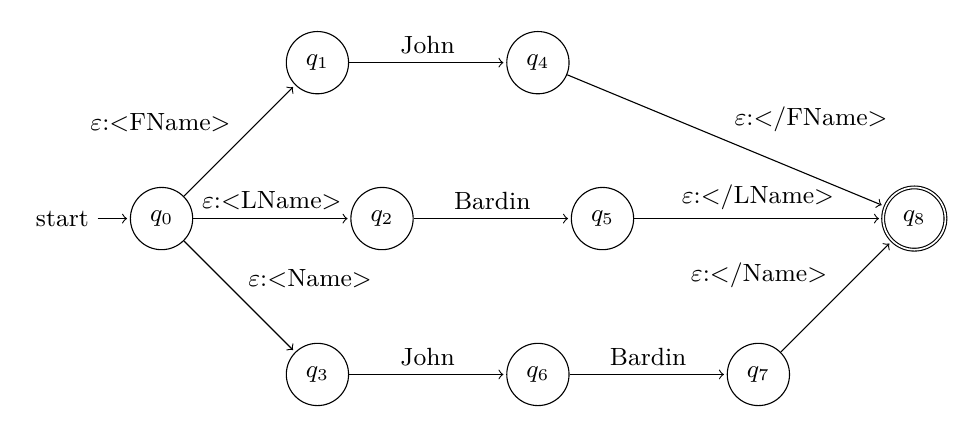
\begin{tikzpicture}[shorten >=1pt,node distance=2.8cm,auto,on grid] 
\small
   \node[state,initial] (q_0)   {$q_0$}; 
   \node[state] (q_1) [above right=of q_0] {$q_1$}; 
   \node[state] (q_2) [right=of q_0] {$q_2$}; 
   \node[state] (q_3) [below right=of q_0] {$q_3$};
   \node[state] (q_4) [right=of q_1] {$q_4$};
   \node[state] (q_5) [right=of q_2] {$q_5$};
   \node[state] (q_6) [right=of q_3] {$q_6$};
   \node[state] (q_7) [right=of q_6] {$q_7$};
   \node[state,accepting] (q_8) [above right=of q_7] {$q_8$};
    \path[->] 
    (q_0) edge  node {$\varepsilon$:<FName>} (q_1)
          edge  node {$\varepsilon$:<LName>} (q_2)
          edge  node {$\varepsilon$:<Name>} (q_3)
    (q_1) edge  node {John} (q_4)
    (q_2) edge  node {Bardin} (q_5)
    (q_3) edge  node {John} (q_6)
    (q_6) edge  node {Bardin} (q_7)
    (q_4) edge  node {$\varepsilon$:</FName>} (q_8)
    (q_5) edge  node {$\varepsilon$:</LName>} (q_8)
    (q_7) edge  node {$\varepsilon$:</Name>} (q_8);
\end{tikzpicture}

In this scenario, every new name is repeated in two places in the network. With
large lists and multiple sources of this type of ambiguity, size inefficiencies
can become serious.

One idea of Pmatch was to recognise the shared prefix in the first name ``John''
and the entire name ``John Bardin'' and to defer tag-writing until the entity
has become unambiguous. In HFST, this is accomplished by detecting the tag directive
during compilation and prefixing the subnetwork in question with an entry marker.
After matching is complete, the entry marker is resolved in linear time with
a simple position stack (in pseudocode):

\begin{verbatim}
for each symbol in result:
    if symbol == entry marker:
         push position into stack
    if symbol is end tag:
         insert corresponding start tag into position at stack top
         pop stack
         append end tag
    else:
         append symbol
\end{verbatim}

With just the entry and end tags, the network simplifies to:

\noindent
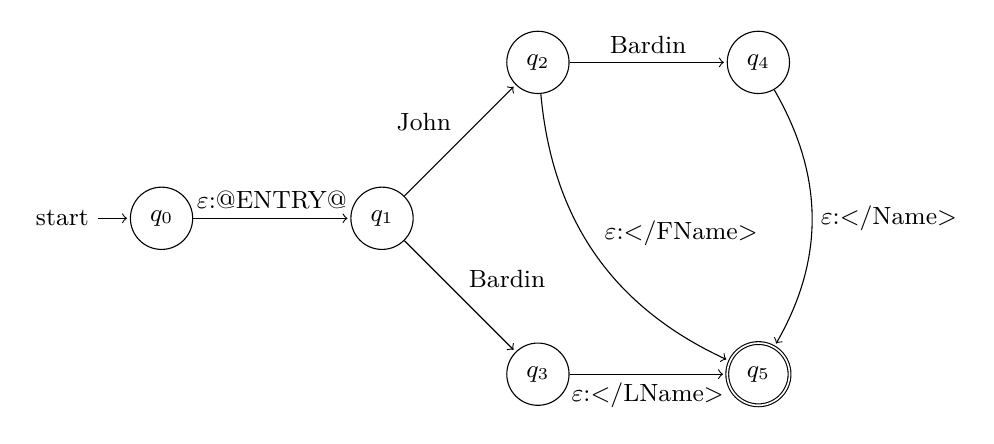
\begin{tikzpicture}[shorten >=1pt,node distance=2.8cm,auto,on grid] 
\small
   \node[state,initial] (q_0)   {$q_0$}; 
   \node[state] (q_1) [right=of q_0] {$q_1$}; 
   \node[state] (q_2) [above right=of q_1] {$q_2$}; 
   \node[state] (q_3) [below right=of q_1] {$q_3$};
   \node[state] (q_4) [right=of q_2] {$q_4$};
   \node[state,accepting] (q_5) [right=of q_3] {$q_5$};
    \path[->] 
    (q_0) edge  node {$\varepsilon$:@ENTRY@} (q_1)
    (q_1) edge  node {John} (q_2)
    (q_1) edge  node {Bardin} (q_3)
    (q_2) edge  node {Bardin} (q_4)
    (q_3) edge [swap] node {$\varepsilon$:</LName>} (q_5)
    (q_2) edge [bend right]  node {$\varepsilon$:</FName>} (q_5)
    (q_4) edge [bend left] node {$\varepsilon$:</Name>} (q_5);
\end{tikzpicture}

\subsubsection{Contexts and States during Matching.}
Context markers trigger special runtime behavior and restrict
progress during matching, very similarly to flag diacritics.
There are two special considerations:

\begin{enumerate}
\item Left contexts are compiled to the left side of the network, in reverse
(so that the first symbol to the left is at the end of the context).
\item Processing direction and position must be preserved during
matching in a state stack.
\end{enumerate}

Additionally, a stack for preserving the input tape position
and the output tape content during each RTN (recursive transition
network) invocation must be kept separately from the runtime
context-checking stack. Otherwise, transition data is not duplicated,
and these stacks are the only arbitrary amounts of memory reserved
for accomplishing non-finite-state extensions.

\subsubsection{Transduction.}
Each matching rule is by default compiled as an identity transduction.
In many applications, however, it is useful to operate on input
with some additional information, but give the output
without such information. Matching is therefore not
performed with automata, but with arbitrary transducers.

\section{Future Work}\label{hfst:discussion}

The idea of combining linguistic rules and statistical models is intriguing but nontrivial.
However, a pure finite-state left-to-right system is likely to be less efficient for
syntactic parsing than a chart-based system, so the solution is probably to add linguistic
constraints in the form of weighted finite-state constraints to a statistical parser before estimating the weights.

% Miikka
While existing statistical models like HMMs and PCFGs can incorporate
a great deal of useful information for tasks like part-of-speech tagging and
syntactic parsing, there are phenomena like non-local congruence which are
too complex to estimate for these models. Probably because of this, there
has been a growing interest in combining rule-based and statistical
methods in core NLP tasks, such as part-of-speech tagging and syntactic
parsing~\cite{manning/2011}. Such a combination presents challenges
both for statistical estimation and inference methods and for the
representation of linguistic information in a way which is compatible
with a statistical system.

Finite-state transducers and automata can be used for expressing
linguistically relevant phenomena for tagging and parsing as regular
string sets. The validity of this approach is demonstrated by the
success of parsing systems like Constraint
Grammar~\cite{karlsson/1990}, which utilizes finite-state
constraints. Weighted machines offer the added benefit of expressing
phenomena as fuzzy sets in a compact way. This makes them an excellent
candidate for adding linguistic knowledge to statistical models.

% NOTE: again, a bit repetitive
\section{Conclusion}\label{hfst:conclusion}
The paper presented various NLP tools implemented with HFST and the minimal extensions they
required to a pure finite-state system. In particular, the paper described an implementation
of a full-scale named-entity recognizer for Swedish using Pmatch achieving a 
10-fold compile-time speed-up compared with the original Flex implementation.

\subsubsection*{Acknowledgments}
The research leading to these results has received funding from FIN-CLARIN, Langnet and the
European Commission's 7th Framework Program under grant agreement n° 238405 (CLARA).


\bibliographystyle{splncs03}
\bibliography{sfcm-2013}

\end{document}
% vim: set spell:
